\documentclass[a4paper,10pt]{article}

% Paquetes requeridos
\usepackage[utf8]{inputenc}
\usepackage[spanish]{babel}
\usepackage{csquotes}
\usepackage{amsmath, amssymb, amsfonts}
\usepackage{graphicx}
\usepackage[style=apa, backend=biber, natbib=true, language=spanish, url=true]{biblatex}
\usepackage{tocloft} % Para personalizar el índice
\usepackage[left=3.5cm,right=2.5cm,top=3.5cm,bottom=3.8cm]{geometry}
\usepackage{setspace} % Espaciado
\usepackage{titlesec} % Para personalizar los títulos
\usepackage{fancyhdr} % Para personalizar encabezados y pies de página
\usepackage{newtxtext}

\pagestyle{fancy}
\fancyhf{} % Limpia encabezados y pies de página
\renewcommand{\headrulewidth}{0pt} % Elimina la línea del encabezado

\addbibresource{referencias.bib}
\DeclareLanguageMapping{spanish}{spanish-apa}
% Configuraciones
\setlength{\parskip}{6pt} % Espacio entre párrafos
\setstretch{1.15} % Espacio entre líneas

\renewcommand{\cftsecleader}{\cftdotfill{\cftdotsep}} % Para puntos en el índice

% Estilos para títulos y subtítulos
\titleformat{\section}
{\normalfont\fontsize{12}{15}\bfseries}{\thesection}{1em}{}
\titleformat{\subsection}
{\normalfont\fontsize{10}{13}\bfseries}{\thesubsection}{1em}{}
\titleformat{\subsubsection}
{\normalfont\fontsize{10.5}{13}\bfseries}{\thesubsubsection}{1em}{}

\usepackage[hypertexnames=false, colorlinks=true, 
linkcolor=blue, 
citecolor=blue, 
urlcolor=blue, 
linkbordercolor={1 1 0}, 
citebordercolor={1 1 0}, 
urlbordercolor={1 1 0}, 
filecolor=blue, 
pdfborderstyle={/S/U/W 1}]{hyperref}

% Inicio del documento
\begin{document}
	\pagestyle{empty}
	% Carátula
	\begin{titlepage}
		\centering
		\vspace*{1.5cm}
		
\includegraphics[width=0.3\textwidth]{unerlogo.png}
		\linebreak
		{\fontsize{14}{17}\bfseries Trabajo integrador: Metaverso y Solidity\par}
		{\small Martín Borgo\par}
		{\small Leandro Molina\par}
		{\normalsize Universidad Nacional de Entre Ríos\par}
		{\normalsize Facultad de Ciencias de la Administración\par}
		{\normalsize Licenciatura en Sistemas \par}
		{\small \href{mailto:martinborgo8@gmail.com}{martinborgo8@gmail.com}\par}
		{\small \href{mailto:LeandroRodrigoMolina@gmail.com}{LeandroRodrigoMolina@gmail.com}\par}
		
		% Resumen y palabras clave
		{\small \textbf{Abstract.} Resumen hasta 200 palabras. \par}
		{\small \textbf{Keywords:} Metaverso, Solidity, Contratos inteligentes (Smart Contracts), Blockchain.\par}
	\end{titlepage}
	
	%Empezamos a escribir
	\section{Introducción}
	El metaverso, conocido también como universo metafísico o espacio virtual, se refiere a un entorno virtual 3D en línea, donde todos los eventos que ocurren en él se producen en tiempo real y tienen un impacto permanente. La palabra “metaverso” está compuesta por el prefijo “meta”, que viene del griego \( \mu\varepsilon\tau\acute{\alpha} \) y significa “más allá” o “después”. En el contexto del metaverso, este prefijo se refiere a la idea de un universo que va más allá de lo físicamente conocido. Por otro lado, el final “-verso” proviene del latín “universus”, que significa “todo en uno” o “entero”. Por lo tanto, el metaverso se puede interpretar como “un universo alternativo” o “más allá del universo”, refiriéndose a un espacio virtual en línea autónomo que existe más allá de nuestro universo físico.
	
	El término metaverso se popularizó por la novela de Neal Stephenson “Snow Crash”, en esta novela de género ciencia ficción, más específicamente del subgénero Cyberpunk\footnote{El subgénero Cyberpunk se centra en futuros distópicos donde hay tecnología avanzada y todo lo relacionado a la computación está conectado a una sociedad en decadencia. Ejemplos del subgénero Cyberpunk pueden ser: Neuromancer, Akira, Matrix, Cyberpunk 2077, etc.}. En la novela de Neal, el metaverso es un espacio virtual donde las personas representadas por avatares, interactúan, socializan y hacen negocios, es una mezcla de realidad física y realidad virtual. En este mundo se presenta a una sociedad decadente, donde las personas viven en condiciones precarias, y hacen uso del metaverso para escapar de la realidad, las personas pueden crear avatares siendo versiones idealizadas de ellos mismos, interactuar con entornos limpios y ordenados, participar en actividades que no pueden realizarse en la vida real. Además de utilizarse como medio de comunicación, educación, comercio, etc.
	
	El término metaverso se popularizó con “Snow Crash”, pero este término no fue usado por primera vez por Neal, este ya existía desde antes, por ejemplo en 1980 William Gibson escribió “Neuromancer” donde se presentaba un concepto similar. Es interesante la evolución del término metaverso, ya que este nació en la literatura Cyberpunk para los futuros distópicos de sus novelas y ha avanzado con el paso del tiempo a una definición formal y con tecnologías en la vida real que ya estamos viendo actualmente.
	
	Desde 1992 el metaverso se fue desarrollando constantemente podemos dividir su evolución en cuatro etapas:
	\begin{enumerate}
		\item Etapa Embrionaria (1992-2007): Basada en literatura y arte.
		\item Etapa Primaria (2008-2013): Basado en videojuegos.
		\item Etapa de Reflujo (2014-2019): Restringida por muchos problemas abiertos.
		\item Etapa de Desarrollo (2020-actualidad): Integración de diversas tecnologías para lograr aplicaciones en múltiples campos.
	\end{enumerate}
	
	En estas etapas las podemos ver en el número de publicaciones a lo largo de los años, usando bases de datos como Web of Science y Scopus. Web of Science hasta 1 de noviembre 2021, se han publicado  en total 211 relacionadas con el metaverso mientras que Scopus un total de 191 publicaciones. Las publicaciones por año van incrementado en este tema, con cada vez más desarrollo de esta tecnología:
	%\( \mu\varepsilon\tau\acute{\alpha} \)
	\begin{figure}[h]
		\centering
		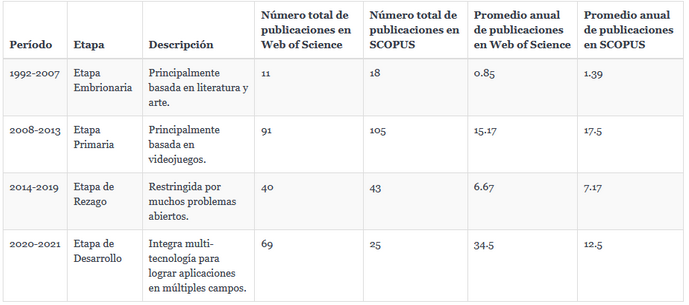
\includegraphics[width=0.7\textwidth]{tablaPublicaciones.PNG}
		\caption{Hecho en base de \textcite{ning2023survey}}
		\label{fig:tabla_publicaciones}
	\end{figure} \\
	Actualmente estamos en la etapa de desarrollo donde se están integrando y desarrollando diferentes tecnologías para la creación del Metaverso.  Estas tecnologías se pueden dividir en cinco aspectos: infraestructura de red, tecnología de gestión, tecnología común básica, conexión de objeto de realidad virtual y convergencia de realidad virtual. Una breve descripción de las tecnologías involucradas es la siguiente:

	\begin{enumerate}
		\item \textbf{Infraestructura de comunicación y computación:} Se refiere a las bases tecnológicas que hacen posible el Metaverso, principalmente las redes 5G y 6G. Estas redes ofrecen alta velocidad, baja latencia y conectividad ubicua. La comunicación cuántica garantiza la seguridad en este entorno. Además, el Internet de las Cosas (IoT) es esencial para conectar el Metaverso con el mundo real. La computación en la nube y en el borde son fundamentales para proporcionar la potencia informática necesaria.
		\item \textbf{Tecnología de Gestión:} Se centra en cómo se gestionan y mantienen los recursos dentro del Metaverso. Esto incluye la gestión de la energía utilizada por las instalaciones del Metaverso, la asignación y descubrimiento de recursos y la gestión de las interacciones de los usuarios en sesiones. La seguridad y la prevención de ataques también son consideraciones clave en este ámbito.
		\item \textbf{Tecnologías fundamentales:} Son las tecnologías esenciales que respaldan las operaciones y el desarrollo del Metaverso. Estas incluyen la realidad virtual y aumentada, la inteligencia artificial, la visión por computadora y la tecnología blockchain. Estas tecnologías permiten la creación de mundos virtuales y la interacción dentro de ellos. Entre ellas IA con frameworks como TensorFlow, permitiendo interacciones avanzadas, lenguajes como Solidity respalda contratos inteligentes y transacciones seguras.
		\item \textbf{Conexión de Objetos de Realidad Virtual:} Trata sobre cómo los objetos virtuales en el Metaverso interactúan entre sí y con los usuarios. Esto abarca desde la creación de objetos hasta su interacción y eventual destrucción, todo lo cual contribuye a una experiencia inmersiva para los usuarios.
		\item \textbf{Convergencia de Realidad Virtual:} Se refiere a la interacción entre el mundo virtual del Metaverso y el mundo real. Esto incluye cómo la información se mueve entre estos dos mundos, cómo los usuarios pueden transitar entre ellos y cómo las acciones en uno pueden influir en el otro. Por ejemplo, cómo las tecnologías AR (Augmented Reality), VR (Virtual Reality), MR (Mixed Reality).
	\end{enumerate}
	Las tecnologías emergentes como la realidad virtual (VR) y la realidad aumentada (AR) y las demás tecnologías mencionadas anteriormente están impulsando el desarrollo del metaverso, abriendo nuevas oportunidades en mercados y entretenimiento previamente inexplorados o de nicho. Esto incluye el comercio de bienes virtuales y la experiencia de eventos históricos de formas novedosas. 
	Sin embargo, el camino hacia un metaverso completamente desarrollado enfrenta obstáculos significativos, incluyendo desafíos técnicos, éticos y de salud mental, así como cuestiones de interoperabilidad y compatibilidad.\newline
	En este trabajo, nos centraremos principalmente en explorar el papel del lenguaje de programación Solidity (viendo diferentes aplicaciones del mismo), central para la implementación de los contratos inteligentes y la blockchain, se lo puede considerar dentro del backend del metaverso, dejando de lado la discusión detallada de otros conceptos clave\footnote{Para ver una descripción clara de estos términos véase: \textcite{grandury2022implementacion}}.
	\section{Desarrollo de trabajo}
	En este apartado 
	\subsection{La Blockchain en el Metaverso}
	La tecnología blockchain y sus herramientas afines, como los contratos inteligentes, no solo establecen los cimientos de una economía tangible en el metaverso, sino que también tienen el potencial de mejorar significativamente la seguridad y la integridad de los datos. \textcite{huynh2023blockchain} hablan de como la adquisición de datos en el metaverso es algo fundamental, sobre todo en el entrenamiento de inteligencia artificial o algoritmos de aprendizaje automáticos. Para que todo eso sea posible se requiere información útil y auténtica, en este artículo se discute cómo la tecnología blockchain facilita esta tarea. Por un lado, esta tecnología hará que cada uno de los usuarios tengan control sobre su propia información, pudiendo transferir y compartir esta con terceras partes a través de un contrato inteligente y por otro lado al estar toda esta información en la cadena de bloques nos aseguramos que esta mismo es completamente auténtica y totalmente útil.
	
	Existen ya una variedad de trabajos que exploran los posibles usos de los contratos inteligentes aplicados sobre todo a la transferencia y protección de datos. \textcite{liu2018enforceable} presenta un marco de trabajo para la transferencia de información y el acceso a datos utilizando contratos inteligentes. A grandes rasgos, los investigadores proponen un proceso en el que las partes acuerdan términos por fuera de la cadena de bloques, crean un contrato inteligente personalizado según esos términos, proporcionando un enlace de acceso único a la parte demandante que le permitirá acceder a los datos guardados en la nube. Si alguna de las partes no cumple con los términos, se recurre a un 'congreso', un contrato inteligente de votación en el que un jurado decide si hubo un incumplimiento y en caso de que sea necesario se aplica una multa. Algo muy similar es propuesto por \textcite{ouyang2020learning} que presenta un marco de trabajo basado en Federal Learning y contratos inteligentes para entrenar de forma totalmente descentralizada y segura a los algoritmos de inteligencia artificial y aprendizaje automático. En el mismo artículo se menciona el concepto de “Mercados de aprendizaje”, donde las distintas partes que entrenan a los modelos de IA pueden comercializar los resultados obtenidos del entrenamiento.
	
	Este tipo de marcos de trabajos representan una gran avance para el metaverso, ya que la inteligencia artificial se presenta como una herramienta esencial que potenciará la inmersión de estos mundos virtuales. Desempeñando un papel clave en la personalización de entornos virtuales, la interacción con usuarios, la simulación de mundos virtuales realistas. De ahí que hayan surgido una infinidad de trabajos que exploran los usos de la inteligencia artificial, un ejemplo es el trabajo realizado por \textcite{yang2022fusing} donde se discute de cómo los NPCs conducidos por inteligencia artificial pueden, mediante el entrenamiento adecuado, adaptarse a cualquier rol que se les quiera asignar. El mismo artículo da el ejemplo como se realizó un experimento donde se entrenó a OpenAI 5 durante 10 meses en Dota 2, logrando ésta derrotar a los campeones mundiales de ese año en una partida, demostrando que con el entrenamiento adecuado la inteligencia artificial puede tener el mismo rendimiento que los seres humanos en la realización de tareas difíciles. Ya dándole un propósito más específico \textcite{hwang2022definition} en su artículo propone la creación de NPCs impulsados por IA con fines educativos, concretamente los autores mencionan 3 roles que pueden desempeñar estos NPCs, en primer rol es el de profesor, en segundo rol es el de alumno, que resulta útil para realizar capacitaciones docentes o incluso para generar una retroalimentación al estudiante por parte de otros estudiantes. El tercer rol es el de par, el cual está más orientado al apartado de simulación de entornos o recreación de escenarios, algo extremadamente útil para el área médica y militar, entre muchas otras.
	
	\subsection{Solidity y los Smart Contracts}
	
	\section{Resultados obtenidos}
	\section{Conclusiones}
	\nocite{*}
	\printbibliography[heading=bibintoc]
\end{document}
